
\documentclass[sigconf,nonacm]{acmart}
\usepackage{graphicx}
\usepackage{rotating}
\usepackage{tikz}
\usetikzlibrary{positioning, arrows.meta, fit, backgrounds, calc}

\settopmatter{printacmref=false, printfolios=false}
\setcopyright{none}
\renewcommand\footnotetextcopyrightpermission[1]{}
\pagestyle{plain}
\begin{document}

\title{RepNet Progress Report - April 17, 2026}

\author{Ahmed Khan}
\email{aekhan@ucdavis.edu}
\affiliation{%
  \institution{UC Davis}
  \city{Davis, CA}
  \country{USA}
}

\author{Lawrencedel Legaspi}
\email{lawlegaspi@ucdavis.edu}
\affiliation{%
  \institution{UC Davis}
  \city{Davis, CA}
  \country{USA}
}

\author{Selena Phu}
\email{slphu@ucdavis.edu}
\affiliation{%
  \institution{UC Davis}
  \city{Davis, CA}
  \country{USA}
}

%%
%% This command processes the author and affiliation and title
%% information and builds the first part of the formatted document.
\maketitle

\section{Introduction}
Risk Estimation of Preeclampsia Network (RepNet) is our research in improving the classification of 12-Lead electrocardiogram (ECG) waveforms for estimation of preeclampsia. We aim to do this via a transformer based convolutional neural network (CNN) trained on a proprietary UC Davis Health (UCDH) dataset. We aim to augment dataset imbalance using a transformer based generative adversarial network (GAN). We will explore the only one past work done on this specific subject and make advancements on the foundation of their work, and benchmark against it. We will also explore the retraining of an existing ECG large foundation model (LFM) as well as benchmarking against their performance versus our specific architecture. We aim to bolster clinical interpretability through attention mapping of the neural network. And lastly we aim to train a random forrest (RF) classifier and visualize manually extracted ECG features from the RF classifier alongside the attention mapping of deep learning to augment clinical workflows by providing explainability to clinicians, assinging quantities to qualia.


\section{Review of the Literature}

We performed a review of the literature by first querying ChatGPT, which performed broad internet searches over academic archives such as PubMed, Google Scholar, ArXiv, etc. We queried it for ranking the best papers across specific fields we intend to study, such as the state of the art of machine learning (ML) models for preeclampsia or deep learning for the entire field of ECG classification. Papers were evaluated based on their bredth, rigor, and relevance to a novel research project. After this review of literature reviews, we intend to select the most relevant original studies each mention for our actual deep dive into model architecture and methods whilst doing development and validation, and such will be reported in Progress Report 2. See appendix A for the list of reviewed literature.

\subsection{Preeclampsia ML Literature Reviews}

We sought a comprehensive review over the field machine learning and deep learning research into preeclampsia, to see what work had been done to solve this problem in the past. We selected Özcan et al. as it both a broad overview across classical ML and modern DL, a review of specific papers and the trade offs of their models. Ozcan included 35 papers published from 2018 to 2023 [cite]. It serves as a good primer into the state of the art. We also selected a statistical meta-analysis by Liu et al that goes much deeper into comparison of model performance between a smaller number of 26 papers [cite].

None of the models presented in Özcan et al or Liu et al were trained to classify ECG waveforms in any way, they were all various methods of learning from other features such as electronic health record (EHR) data and risk factors [ double cite ] . To our knowledge there is only one relevant previous work, Butler et al which showcases a 1-D CNN they call ECG-AI [cite]. There is also an older study by Euliano et al which is on 3-Lead instead of 12-Lead ECG and they perform linear descriminant analysis (LDA), a classical ML approach [cite].

By extension, the reviews do not showcase any decision tree (DT) type models to classify ECG Waveforms of preeclampsia, though many RF models exist using other features such as EHR data. We further confirm this by an extended-thinking ChatGPT query, asking it to return all ECG Waveform ML papers on preeclampsia besides Butler et al and it comes up blank. This indicates that the field of both classical ML and modern DL on ECG waveforms of preeeclampsia is an untapped research field that is ripe for contribution.

\subsection{ECG Classification ML Literature Reviews}

In the general field of ECG Waveform classification, we selected the literature review by Boulif et al as a broad scope primer that covers both ML and DL methods [cite]. We also selected Prakash et al as a deep systematic review that covers much more research process and model architecture [ cite ].

Since we are focusing on cutting edge DL such as CNN enhanced by attention mechanisms, we selected M Ansari et al for its comprehensive survey of transformers and LLMs specifically [ cite ]. Furthermore we selected Y Ansari et al for its deep systematic analysis and cmparison of DL model architectures [cite].

\subsection{ECG Classification Large Foundation Models}

LFM's hold promise for their training on millions of ECG waveforms, they save us the trouble of access to limited data by training the earlier layers on massive amounts of data, giving it robust feature extraction that can then be reasoned about for different classification tasks after the fact [cite] We selected Han et al. as the leading literature review on ECG Classification LFM's. Picking a specific model to work with, we selected ECG-Founder since it is the leading performance in the field, they provide a GitHub repository with all relevant infrastructure and pipelines such as signal preprocessing and running benchmarks on public datasets [cite]. We will compare our model's performance trained on these public datasets as well as a fine tuned ECG-Founder against our special purpose model.

\subsection{ECG Waveform Features of Preeclampsia}

Since our RF model will train on manual featurization on ECG waveforms, we will explore relevant papers. We selected older papers firmly in the camp of clinical electrocardiography rather than machine learning or deep learning. Angeli et al serves a review of a few ECG features of preeclampsia [cite]. Rafaelli et al deep dives into a single feature, the most prominently noted QT interval, with visual and mathematical analysis as a demonstration of the approach for the other features we have been assigned or find relevant in the literature [cite].

\subsection{Reviews of Preprocessing ECG Waveforms}

ECG waveforms are subject to noise from environmental factors such as improper adhesion of contacts, movement during treatment, inductive interference from power lines, and the subtle differences in the real world electrical components such as DACs that convert signals to data [cite]. We have selected Jia et al as an overview of data preprocessing techniques that we can collectively employ across our models and evaluating which combination leads to the best results [cite]. Most literature build off of a standard approach first doing baseline wander highpass filtering and z-score normalization, sometimes notch filtering the 50 hz (world) or 60 hz (USA) powerline interference [cite]. To shift left our preprocessing quality evaluation before model training and validation, to save much time and compute on experiment, we selected Satija et al which covers methods for ECG signal quality assessment [cite].

\subsubsection{Preeclampsia Decision Tree Classification}
Since we are training a RF classifier, a variant of decision tree, and furthermore performing dimensionality reduction on ECG leads, we selected Musa et al as they performed an original study of PCA on a DT classifier for preeclampsia, which may indicate how we approach having a dimensionally reduced feature set input for our RF classifier [cite].

We also selected Park et al, an original study which performed DT classification for ECG waveforms [cite]. We feel that these papers combined serve as a foundation for how we approach the deeper aspects of our preeclampsia ECG RF classifier, and how it may incorporate other dimensions such as EHR data.

\subsection{Data Augmentation for ECG Waveforms}
An endemic issue of medical ML is sparse access to datasets, which themselves are small and restricted access, especially for lesser researched diseases that would benefit from such work [cite] Furthermore, such datasets have a wild class imbalance because there is no guarantee that diseases are an ideal 50\% of the sample population, diseased sample points are usually in the minority [cite].

Data balancing such as majority undersampling are severely detrimental for throwing away a large portion of the usable data and restricting to an extremely small dataset, and minority oversampling does not really solve anything as simply reasserting the same points does not generalize to learning the decision surface, and may cause the model to overfit [cite]. We selected an overview of ECG data augmentation strategies by Rahman et al.

There are more advanced data augmentation strategies that try to interpolate points on the data manifold, such as synthetic minority oversampling technique (SMOTE) [cite]. Then there are GAN models that try to infer the structure of the data manifold in a nonlinear way through training a generator and descriminator, with the descriminator trying to distinguish synthetic from actual points, and the generator trying to be less perceptable to the descriminator, and it ends up creating sample points that are more indicative of the dataset, and this helps the model train better [cite]. We selected a paper by Xia et al on transformer based GAN for boosting datasets ECG classification [cite].

\subsection{ECG Model Efficiency and Compression}
After we have trained a performant model, we must tackle the challenge of deployment on edge devices. Not every clinical setting has direct access to a dedicated compute cluster or server, in general it is expected for the diagnostic tool to be self contained. Medical privacy protections prevent such data from being transmitted to cloud compute solutions [cite]. Furthermore, consider compute constraints for financial reasons, such as smaller clinics or even the developing world where preeclampsia disproportionately kills. It would be useful to deploy if we could achieve a model of similar performance for a fraction of the memory and compute costs [cite].

We selected Gupta et al as it is specifically a literature review on efficient ECG Classification models, both existing efficient architectures and strategies to shrink models such as distillation, quantization, pruning, etc [cite]. We also selected Keivanimehr as it covers TinyML for ECG classification. TiyML is a framework for deploying machine learning on edge and embedded devices, and as such we woul explore how to fit our model into this framework [cite]

\subsection{Capstone Project Assigned Literature}
In our initial assignment of the capstone project, we were given four papers to read, as an introduction to certain concepts that are meant to guide our direction of research [cite proj assign] They appear to fall into two camps.

\subsubsection{Machine Learning for ECG or Preeclampsia}
We were provided Joshi et al, an associate of Professor Chuah that runs the Rubinet lab that the RepNet research project is under. Joshi et al performed the same bicameral machine learning approach that we are instructed to do, training both a RF classifier and a CNN model on a public regional wall motion abnormality (RWMA) dataset [cite]. We were also provided Butler et al, it is to date the only previous attempt at creating a DL model for preeclampsia ECG waveforms, and we seek to advance the field upon this valuable exploratory work, it cannot be overstated where credit is due [cite]. Butler's relevance to our research will be elaborated upon in a subsequent section.

\subsubsection{Dimensionality Reduction in Leads}

We were provided Xue et al which covers dimensionality reduction in the ECG channels and if they still contain the relevant information and if they can be reconstructed with interpolation [cite]. We were also provided Attia et al that explores ECG classification from a single lead, showing what is possible at the limit of the dimensionality reduction [cite]. Dimensionality reduction is relevant because a fully-kitted 12 Lead ECG is still the most extreme measure, used in large hospitals. In any situation such as for paramedics, smaller clinics, or even the developing world where preeclampsia disproportionately kills, it would be useful to still be able to draw conclusions even with constrained diagnostic resources [cite].

\section{Butler et al ECG-AI Architecture and Weights}
We have obtained the model dimensions and weights of the ECG-AI trained by Butler et al. from his colleague's GitHub. This model can serve as a benchmark against our own model, both in the performance of their model weights, and the performance of their model architecture trained on our dataset. Furthermore, the architecture serves as a starting point where we can experiment with transfer learning in freezing in retraining different layers, append, pre-pend, replace, or shim layers to achieve new functions such as attention, all in the aim of even better performance.

\subsection{ECG-AI Model Architecture}

The Butler et al.\ ECG-AI model is a 1-D residual convolutional neural network that accepts 12-lead ECG signals of length 2250 samples. The architecture comprises six residual blocks organized into three stages of progressively increasing filter width (16, 32, 64), each followed by max-pooling and dropout for regularization. A final flatten and dense softmax layer produces a two-class output. Figure~\ref{fig:butler-arch} summarizes the architecture; see Appendix~B for the full decomposed layer-by-layer model architecture.

% --- Figure 1: High-level ResBlock summary ---
\begin{figure}[h]
\centering
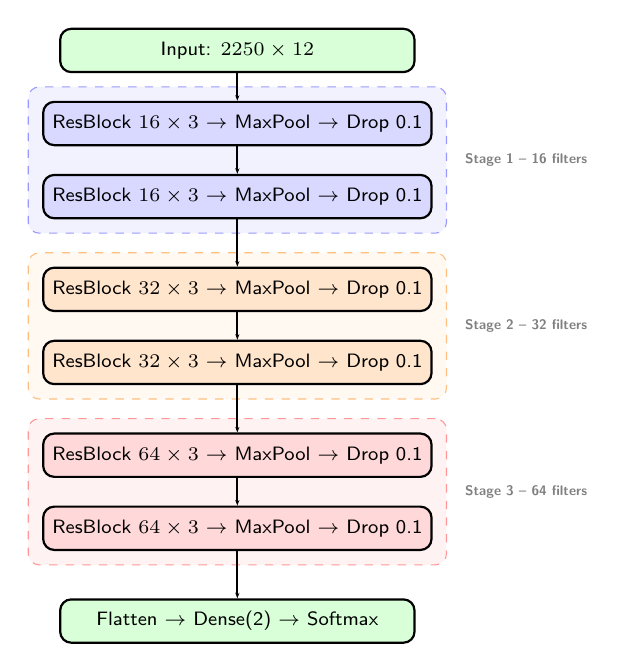
\begin{tikzpicture}[
    node distance=0.35cm,
    block/.style={draw, rounded corners, minimum height=0.55cm, minimum width=4.5cm,
                  font=\scriptsize\sffamily, align=center, thick},
    stage16/.style={block, fill=blue!15},
    stage32/.style={block, fill=orange!20},
    stage64/.style={block, fill=red!15},
    io/.style={block, fill=green!15},
    arrow/.style={-{Stealth[length=2pt]}, thick},
    stagelabel/.style={font=\tiny\sffamily\bfseries, text=gray},
]

\node[io] (input) {Input: $2250\times12$};
\node[stage16, below=of input] (rb1) {ResBlock $16\times3$ $\to$ MaxPool $\to$ Drop 0.1};
\node[stage16, below=of rb1] (rb2) {ResBlock $16\times3$ $\to$ MaxPool $\to$ Drop 0.1};
\node[stage32, below=0.6cm of rb2] (rb3) {ResBlock $32\times3$ $\to$ MaxPool $\to$ Drop 0.1};
\node[stage32, below=of rb3] (rb4) {ResBlock $32\times3$ $\to$ MaxPool $\to$ Drop 0.1};
\node[stage64, below=0.6cm of rb4] (rb5) {ResBlock $64\times3$ $\to$ MaxPool $\to$ Drop 0.1};
\node[stage64, below=of rb5] (rb6) {ResBlock $64\times3$ $\to$ MaxPool $\to$ Drop 0.1};
\node[io, below=0.6cm of rb6] (flat) {Flatten $\to$ Dense(2) $\to$ Softmax};

\foreach \a/\b in {input/rb1, rb1/rb2, rb2/rb3, rb3/rb4, rb4/rb5, rb5/rb6, rb6/flat}{
    \draw[arrow] (\a) -- (\b);
}

\begin{scope}[on background layer]
    \node[fit=(rb1)(rb2), inner sep=5pt, draw=blue!40, fill=blue!5, rounded corners, dashed] (s1) {};
    \node[stagelabel, right=3pt of s1] {Stage 1 -- 16 filters};
    \node[fit=(rb3)(rb4), inner sep=5pt, draw=orange!50, fill=orange!5, rounded corners, dashed] (s2) {};
    \node[stagelabel, right=3pt of s2] {Stage 2 -- 32 filters};
    \node[fit=(rb5)(rb6), inner sep=5pt, draw=red!40, fill=red!5, rounded corners, dashed] (s3) {};
    \node[stagelabel, right=3pt of s3] {Stage 3 -- 64 filters};
\end{scope}

\end{tikzpicture}
\caption{High-level view of the Butler et al.\ ECG-AI architecture showing six ResBlocks (Figure~\ref{fig:resblock}) across three filter-width stages (filter widths 16, 32, 64), each stage followed by max-pooling and dropout, culminating in a dense softmax output layer.}
\label{fig:butler-arch}
\end{figure}

% --- Figure 2: ResBlock internal structure ---
\begin{figure}[h]
\centering
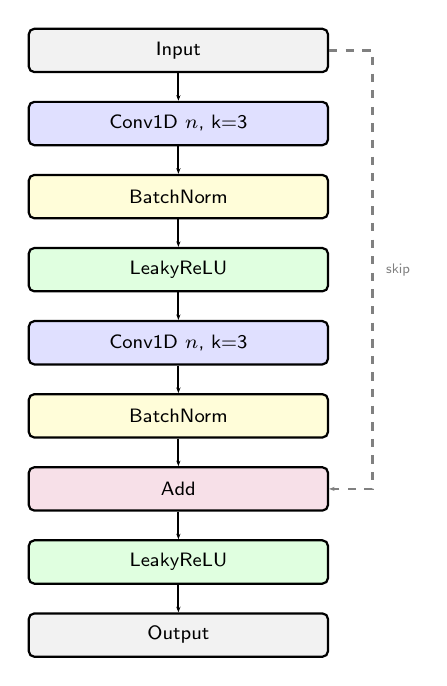
\begin{tikzpicture}[
    node distance=0.35cm,
    block/.style={draw, rounded corners=2pt, minimum height=0.55cm, minimum width=3.8cm,
                  font=\scriptsize\sffamily, align=center, thick},
    conv/.style={block, fill=blue!12},
    bn/.style={block, fill=yellow!15},
    act/.style={block, fill=green!12},
    addn/.style={block, fill=purple!12},
    arrow/.style={-{Stealth[length=2pt]}, thick},
    skiparrow/.style={-{Stealth[length=2pt]}, thick, dashed, gray},
]

\node[block, fill=gray!10] (input) {Input};
\node[conv, below=of input] (c1) {Conv1D $n$, k=3};
\node[bn, below=of c1] (b1) {BatchNorm};
\node[act, below=of b1] (a1) {LeakyReLU};
\node[conv, below=of a1] (c2) {Conv1D $n$, k=3};
\node[bn, below=of c2] (b2) {BatchNorm};
\node[addn, below=of b2] (add) {Add};
\node[act, below=of add] (a2) {LeakyReLU};
\node[block, fill=gray!10, below=of a2] (output) {Output};

% Sequential arrows
\foreach \a/\b in {input/c1, c1/b1, b1/a1, a1/c2, c2/b2, b2/add, add/a2, a2/output}{
    \draw[arrow] (\a) -- (\b);
}

% Skip connection on the right
\draw[skiparrow] (input.east) -- ++(0.55,0) |- (add.east);

% Label the skip
\node[font=\tiny\sffamily, text=gray, right=0.6cm of a1] {skip};

\end{tikzpicture}
\caption{Internal structure of a ResBlock. The skip connection bypasses two Conv1D--BatchNorm--LeakyReLU pairs. A $1\times1$ projection is applied on the skip path at stage boundaries to match filter dimensions.}
\label{fig:resblock}
\end{figure}

\appendix
\clearpage
\onecolumn
\section{Summary of Reviewed Literature}

\begin{table*}[h]
\caption{Summary of Reviewed Literature}
\label{tab:literature}
\small
\centering
\begin{tabular}{p{0.28\textwidth}p{0.14\textwidth}p{0.48\textwidth}}
\toprule
\textbf{Paper} & \textbf{Type} & \textbf{Purpose} \\
\midrule
\multicolumn{3}{l}{\textit{Preeclampsia ML Literature Reviews}} \\
Özcan et al. & Review & General overview of ML models in preeclampsia \\
Liu et al. & Review & \\
\midrule
\multicolumn{3}{l}{\textit{ECG Classification ML Literature Reviews}} \\
Boulif et al. & Review & Broad overview of ECG classification methods \\
Prakash et al. & Review & Systematic review of ML and DL for ECG beat classification \\
Y. Ansari et al. & Review & Overview of DL architectures for ECG (2017-2023) \\
M. Ansari et al. & Review & Survey of transformers and LLMs for ECG processing \\
\midrule
\multicolumn{3}{l}{\textit{ECG Classification Large Foundation Models}} \\
Han et al. & Review & Review of large foundation models for ECG \\
McKeen et al. & Original & ECG-FM open source foundation model \\
\midrule
\multicolumn{3}{l}{\textit{ECG Waveform Features of Preeclampsia}} \\
Rafaelli et al. & Original & ECG features of preeclampsia \\
Angeli et al. & Original & QT interval relevance for preeclampsia \\
\midrule
\multicolumn{3}{l}{\textit{Reviews of Preprocessing ECG Waveforms}} \\
Jia et al. & Review & Overview of ECG preprocessing techniques \\
Satija et al. & Review & ECG signal quality assessment \\
\midrule
\multicolumn{3}{l}{\textit{Preeclampsia Decision Tree Classification}} \\
Park et al. & Original & Decision tree methods on ECG waveforms \\
Musa et al. & Original & PCA on decision tree classifier for preeclampsia \\
\midrule
\multicolumn{3}{l}{\textit{Data Augmentation for ECG Waveforms}} \\
Rahman et al. & Review & Overview of ECG data augmentation \\
Xia et al. & Original & Transformer GAN for data augmentation \\
\midrule
\multicolumn{3}{l}{\textit{ECG Model Efficiency and Compression}} \\
Gupta et al. & Review & Efficient model design for ECG classification \\
Keivanimehr et al. & Original & Model compression for ECG classification \\
\midrule
\multicolumn{3}{l}{\textit{Capstone Project Assigned Literature}} \\
Butler et al. & Original & 1-D CNN for preeclampsia ECG classification \\
Xue et al. & Original & ML methods for preeclampsia prediction \\
Attia et al. & Original & ML applications in ECG analysis \\
Joshi et al. & Original & Lead reduction in ECG analysis \\
\bottomrule
\end{tabular}
\end{table*}

\clearpage
\section{Butler et al. Full Layer-by-Layer Architecture}
\vspace{1em}
\noindent\centering
\resizebox{!}{0.75\textheight}{%
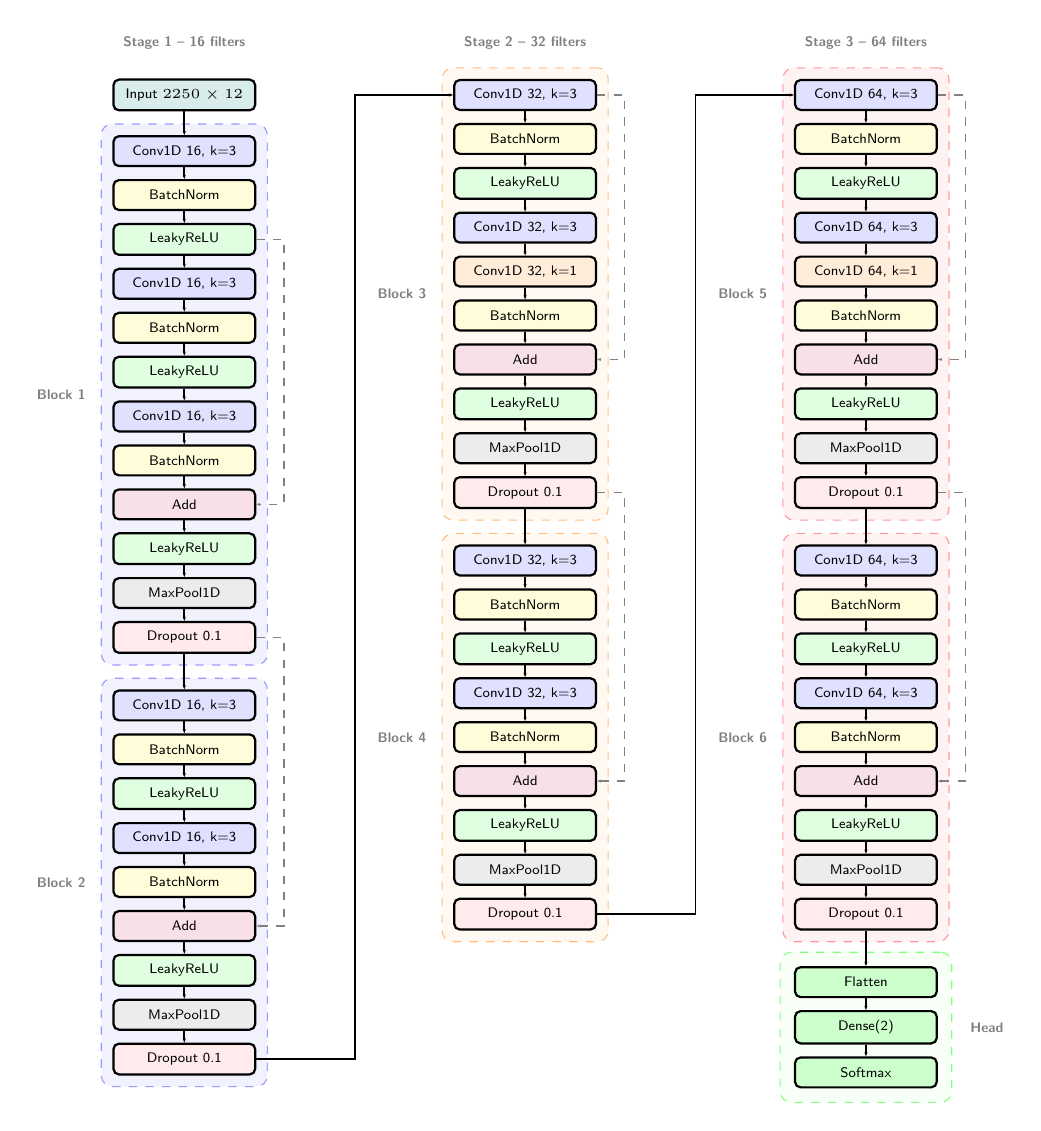
\begin{tikzpicture}[
    node distance=0.15cm,
    layer/.style={draw, rounded corners=2pt, minimum height=0.38cm, minimum width=1.8cm,
                  font=\tiny\sffamily, align=center, thick},
    conv/.style={layer, fill=blue!12},
    bn/.style={layer, fill=yellow!15},
    act/.style={layer, fill=green!12},
    add/.style={layer, fill=purple!12},
    pool/.style={layer, fill=gray!15},
    drop/.style={layer, fill=red!8},
    head/.style={layer, fill=green!20},
    io/.style={layer, fill=teal!15},
    proj/.style={layer, fill=orange!15},
    arrow/.style={-{Stealth[length=1.5pt]}, semithick},
    skiparrow/.style={-{Stealth[length=1.5pt]}, semithick, dashed, gray},
    stagelabel/.style={font=\tiny\sffamily\bfseries, text=gray},
]

% ---- Column 1: Blocks 1-2 (16 filters) ----
\node[io] (in) {Input $2250\times12$};

% Block 1
\node[conv, below=0.3cm of in] (c0) {Conv1D 16, k=3};
\node[bn, below=of c0] (b0) {BatchNorm};
\node[act, below=of b0] (a0) {LeakyReLU};
\node[conv, below=of a0] (c1) {Conv1D 16, k=3};
\node[bn, below=of c1] (b1) {BatchNorm};
\node[act, below=of b1] (a1) {LeakyReLU};
\node[conv, below=of a1] (c2) {Conv1D 16, k=3};
\node[bn, below=of c2] (b2) {BatchNorm};
\node[add, below=of b2] (add0) {Add};
\node[act, below=of add0] (a2) {LeakyReLU};
\node[pool, below=of a2] (mp0) {MaxPool1D};
\node[drop, below=of mp0] (d0) {Dropout 0.1};

% Block 2
\node[conv, below=0.45cm of d0] (c3) {Conv1D 16, k=3};
\node[bn, below=of c3] (b3) {BatchNorm};
\node[act, below=of b3] (a3) {LeakyReLU};
\node[conv, below=of a3] (c4) {Conv1D 16, k=3};
\node[bn, below=of c4] (b4) {BatchNorm};
\node[add, below=of b4] (add1) {Add};
\node[act, below=of add1] (a4) {LeakyReLU};
\node[pool, below=of a4] (mp1) {MaxPool1D};
\node[drop, below=of mp1] (d1) {Dropout 0.1};

% ---- Column 2: Blocks 3-4 (32 filters) ----
\node[conv, right=2.5cm of in] (c5) {Conv1D 32, k=3};
\node[bn, below=of c5] (b5) {BatchNorm};
\node[act, below=of b5] (a5) {LeakyReLU};
\node[conv, below=of a5] (c6) {Conv1D 32, k=3};
\node[proj, below=of c6] (c7) {Conv1D 32, k=1};
\node[bn, below=of c7] (b6) {BatchNorm};
\node[add, below=of b6] (add2) {Add};
\node[act, below=of add2] (a6) {LeakyReLU};
\node[pool, below=of a6] (mp2) {MaxPool1D};
\node[drop, below=of mp2] (d2) {Dropout 0.1};

% Block 4
\node[conv, below=0.45cm of d2] (c8) {Conv1D 32, k=3};
\node[bn, below=of c8] (b7) {BatchNorm};
\node[act, below=of b7] (a7) {LeakyReLU};
\node[conv, below=of a7] (c9) {Conv1D 32, k=3};
\node[bn, below=of c9] (b8) {BatchNorm};
\node[add, below=of b8] (add3) {Add};
\node[act, below=of add3] (a8) {LeakyReLU};
\node[pool, below=of a8] (mp3) {MaxPool1D};
\node[drop, below=of mp3] (d3) {Dropout 0.1};

% ---- Column 3: Blocks 5-6 (64 filters) ----
\node[conv, right=2.5cm of c5] (c10) {Conv1D 64, k=3};
\node[bn, below=of c10] (b9) {BatchNorm};
\node[act, below=of b9] (a9) {LeakyReLU};
\node[conv, below=of a9] (c11) {Conv1D 64, k=3};
\node[proj, below=of c11] (c12) {Conv1D 64, k=1};
\node[bn, below=of c12] (b10) {BatchNorm};
\node[add, below=of b10] (add4) {Add};
\node[act, below=of add4] (a10) {LeakyReLU};
\node[pool, below=of a10] (mp4) {MaxPool1D};
\node[drop, below=of mp4] (d4) {Dropout 0.1};

% Block 6
\node[conv, below=0.45cm of d4] (c13) {Conv1D 64, k=3};
\node[bn, below=of c13] (b11) {BatchNorm};
\node[act, below=of b11] (a11) {LeakyReLU};
\node[conv, below=of a11] (c14) {Conv1D 64, k=3};
\node[bn, below=of c14] (b12) {BatchNorm};
\node[add, below=of b12] (add5) {Add};
\node[act, below=of add5] (a12) {LeakyReLU};
\node[pool, below=of a12] (mp5) {MaxPool1D};
\node[drop, below=of mp5] (d5) {Dropout 0.1};

% Classification head — separate from stages
\node[head, below=0.45cm of d5] (flat) {Flatten};
\node[head, below=of flat] (dense) {Dense(2)};
\node[head, below=of dense] (softmax) {Softmax};

% ---- Sequential arrows within columns ----
% Col 1
\foreach \a/\b in {in/c0, c0/b0, b0/a0, a0/c1, c1/b1, b1/a1, a1/c2, c2/b2, b2/add0, add0/a2, a2/mp0, mp0/d0,
                    d0/c3, c3/b3, b3/a3, a3/c4, c4/b4, b4/add1, add1/a4, a4/mp1, mp1/d1}{
    \draw[arrow] (\a) -- (\b);
}
% Col 2
\foreach \a/\b in {c5/b5, b5/a5, a5/c6, c6/c7, c7/b6, b6/add2, add2/a6, a6/mp2, mp2/d2,
                    d2/c8, c8/b7, b7/a7, a7/c9, c9/b8, b8/add3, add3/a8, a8/mp3, mp3/d3}{
    \draw[arrow] (\a) -- (\b);
}
% Col 3 + head
\foreach \a/\b in {c10/b9, b9/a9, a9/c11, c11/c12, c12/b10, b10/add4, add4/a10, a10/mp4, mp4/d4,
                    d4/c13, c13/b11, b11/a11, a11/c14, c14/b12, b12/add5, add5/a12, a12/mp5, mp5/d5,
                    d5/flat, flat/dense, dense/softmax}{
    \draw[arrow] (\a) -- (\b);
}

% Cross-column arrows — rectangular path between columns
\coordinate (mid12) at ($(d1.east)!0.5!(c5.west)$);
\coordinate (mid23) at ($(d3.east)!0.5!(c10.west)$);
\draw[arrow] (d1.east) -- (mid12 |- d1.east) |- (c5.west);
\draw[arrow] (d3.east) -- (mid23 |- d3.east) |- (c10.west);

% Skip connections (dashed) — routed to the right of each column
\draw[skiparrow] (a0.east) -- ++(0.35,0) |- (add0.east);
\draw[skiparrow] (d0.east) -- ++(0.35,0) |- (add1.east);
\draw[skiparrow] (c5.east) -- ++(0.35,0) |- (add2.east);
\draw[skiparrow] (d2.east) -- ++(0.35,0) |- (add3.east);
\draw[skiparrow] (c10.east) -- ++(0.35,0) |- (add4.east);
\draw[skiparrow] (d4.east) -- ++(0.35,0) |- (add5.east);

% Stage labels at top
\begin{scope}[on background layer]
    % Stage 1 — two res blocks
    \node[fit=(c0)(d0), inner sep=4pt, draw=blue!40, fill=blue!5, rounded corners, dashed] (s1a) {};
    \node[stagelabel, left=2pt of s1a] {Block 1};
    \node[fit=(c3)(d1), inner sep=4pt, draw=blue!40, fill=blue!5, rounded corners, dashed] (s1b) {};
    \node[stagelabel, left=2pt of s1b] {Block 2};
    % Stage 2 — two res blocks
    \node[fit=(c5)(d2), inner sep=4pt, draw=orange!50, fill=orange!5, rounded corners, dashed] (s2a) {};
    \node[stagelabel, left=2pt of s2a] {Block 3};
    \node[fit=(c8)(d3), inner sep=4pt, draw=orange!50, fill=orange!5, rounded corners, dashed] (s2b) {};
    \node[stagelabel, left=2pt of s2b] {Block 4};
    % Stage 3 — two res blocks
    \node[fit=(c10)(d4), inner sep=4pt, draw=red!40, fill=red!5, rounded corners, dashed] (s3a) {};
    \node[stagelabel, left=2pt of s3a] {Block 5};
    \node[fit=(c13)(d5), inner sep=4pt, draw=red!40, fill=red!5, rounded corners, dashed] (s3b) {};
    \node[stagelabel, left=2pt of s3b] {Block 6};
    % Stage group labels — all at same vertical position
    \node[stagelabel, above=3pt of s2a] (s2label) {Stage 2 -- 32 filters};
    \node[stagelabel, above=3pt of s3a] {Stage 3 -- 64 filters};
    \node[stagelabel] at (s1a.north |- s2label) {Stage 1 -- 16 filters};
    \node[fit=(flat)(softmax), inner sep=5pt, draw=green!50, fill=green!3, rounded corners, dashed] (sh) {};
    \node[stagelabel, right=3pt of sh] {Head};
\end{scope}

\end{tikzpicture}%
}
\captionof{figure}{Complete layer-by-layer architecture of the Butler et al.\ ECG-AI model, expanded from Figure~\ref{fig:butler-arch}. The network comprises six residual blocks across three stages of increasing filter width: Stage~1 (16 filters), Stage~2 (32 filters), and Stage~3 (64 filters). Each layer is shown individually --- Conv1D (blue), BatchNorm (yellow), LeakyReLU (green), Add (purple), MaxPool1D (gray), and Dropout (red). Dashed gray arrows indicate residual skip connections that bypass the convolutional layers within each block. Orange blocks denote $1\times1$ projection convolutions at Blocks~3 and~5, where the skip path requires dimensionality matching due to the increase in filter count. The classification head (Flatten, Dense, Softmax) follows after Stage~3.}
\label{fig:butler-detail}

\end{document}
